\section{01 - Intro}

\begin{definition}{Business IT-Risks}
    \begin{itemize}
        \item Ransom Demand
        \item Fraud
        \item Espionage
        \item Violation of Regulations
        \item Misuse of Computing Resources
        \item Reputation Loss
        \item System Outage
        \item Sabotage
        \item Data Loss
        \item Brand Misuse
    \end{itemize}
\end{definition}

\begin{concept}{Problems - Overview} and their impact on data availability
\paragraph{Physisch}
\textbf{unabsichtlich}
\begin{itemize}
    \item Naturkatastrophen
    \item Feuer
    \item Ausfall
    \item Kaffee auf Server
\end{itemize}

\textbf{absichtlich/bösartig}
\begin{itemize}
    \item Feuer
    \item Vandalismus
    \item Garantie läuft aus -> absichtlich langsamer
    \item Social Engineering
\end{itemize}

\paragraph{Virtuell}
\textbf{unabsichtlich}
\begin{itemize}
    \item Bitflip
    \item Config Fehler
    \item Bugs im SW
    \item Phishing klicken
\end{itemize}

\textbf{absichtlich/bösartig}
\begin{itemize}
    \item DDoS
    \item Malware
    \item Ransomware
    \item Phishing senden
    \item Trojaner
\end{itemize}
\end{concept}

\begin{theorem}{Countermeasures - Overview}

\textbf{Disaster Recovery}
    \begin{itemize}
        \item Offline backup solutions
        \item Restoring from images
    \end{itemize}

\textbf{Access Control}
    \begin{itemize}
        \item Restricted Access Rights
        \item Multi-Factor Authentication
        \item Firewalls
        \item Traffic Management Solutions
    \end{itemize}

\textbf{Physical Protection}
    \begin{itemize}
        \item Physical Access Control (locks, fences, etc.)
        \item Fire Protection (extinguishers, alarms, etc.)
        \item Monitoring (CCTV, Guards etc.)
    \end{itemize}

\textbf{Training Processes}
    \begin{itemize}
        \item Employee Training
        \item Four eyes principle
        \item Automation of routine processes
        \item Monitoring
        \item Preventive maintenance
    \end{itemize}

\textbf{Redundancy}
    \begin{itemize}
        \item Uninterruptable Power Supplies
        \item High Availability setups
        \item Load Balancing
        \item Redundant data center
        \item Redundant network connections
    \end{itemize}
\end{theorem}

\begin{formula}{Recovery Plan and Test}

    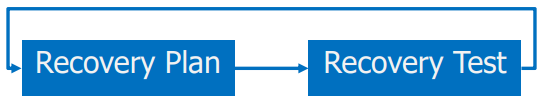
\includegraphics[width=\linewidth]{recovery_plan_test.png}

    \textbf{Recovery Plan} - description of what to do if something goes wrong
    \begin{itemize}
        \item Roles and responsibilities
        \item Processes
        \item Contact details
        \item Technical instructions
    \end{itemize}

    \textbf{Recovery Test} - testing the recovery plan
    \begin{itemize}
        \item Theoretical dry run
        \item Practical tests
        \begin{itemize}
            \item turn off a server or DC
            \item restore data from backup
        \end{itemize}
    \end{itemize}
\end{formula}

\begin{concept}{Goals of IT Security}

Most measures in Information Security have one of the three following high-level goals:
\begin{itemize}
    \item Ensure data is confidential
    \item Ensure data is not corrupted
    \item Ensure data and systems are available
\end{itemize}

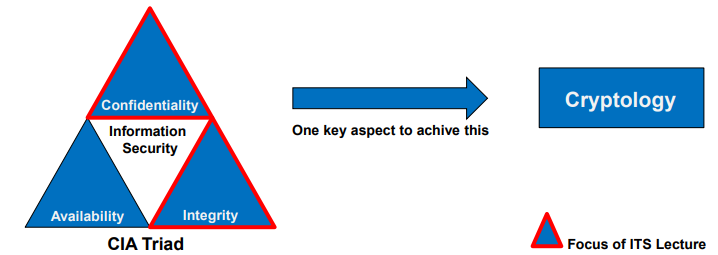
\includegraphics[width=\linewidth]{goals_of_IT_security.png}
\end{concept}